
\chapter{Approach to Molecular Solvents\label{chpt:iem-mdft}}

In the case of non-spherical solvents like water, the solvent particle
carries a molecular structure described by a collection of distributed
atomic interaction sites (LJ and Coulombic). The two theories mentioned
in the previous section are now formulated in the molecular picture
in which each solvent molecule is considered as a rigid body and characterized
by its position $\mathbf{r}$ (e.g. the position of center of mass),
and its orientation $\mathbf{\Omega}$. In \acs{MDFT}, the solvent
is characterized by an angle-dependent inhomogeneous density, $\rho(\mathbf{r},\mathbf{\Omega})$;
in \acs{IET}, an angle-dependent form of the pair distribution function
$g(\mathbf{X}_{1},\mathbf{X}_{2})$ ($X\equiv(\mathbf{r},\mathbf{\Omega})$)
is proposed, while the molecular \acs{OZ} equation is expanded on
rotational invariants. The reference interaction site model (RISM)
\citep{hirata_molecular_2004}, which provides another way for \acs{IET}
to treat molecular solvents, will not be discussed here for the sake of simplicity.

\section{Molecular density functional theory}

In \acf{MDFT}, the free energy functional is rewritten as:
\begin{equation}
\mathcal{F}[\rho(\mathbf{r},\mathbf{\Omega})]=\varOmega[\rho(\mathbf{r},\mathbf{\Omega})]-\varOmega[\rho_{0}]\label{eq:4.grand-pot}
\end{equation}
where $\varOmega[\rho_{0}]$ is the correspondent reference bulk fluid
grand potential at equilibrium. $\rho(\mathbf{r},\mathbf{\Omega})$
is the angle-dependent fluid density function, depending on 3 variables
for spatial coordinates $\mathbf{r}$, and also 3 for orientation
$\mathbf{\Omega}\equiv(\Theta,\Phi,\Psi)$. In the case of linear solvents,
this number can be reduced to 2, i.e. $\mathbf{\Omega}\equiv(\Theta,\Phi)$.
The homogeneous bulk density $\rho_{0}$ is normalized to $n_{0}/\int\mathrm{d}\mathbf{\Omega}$,
to keep coherent with the relation
\begin{equation}
\int\mathrm{d}\mathbf{\Omega}\rho(\mathbf{r},\mathbf{\Omega})=\int\mathrm{d}\cos\Theta\mathrm{d}\Phi\mathrm{d}\Psi\rho(\mathbf{r},\mathbf{\Omega})=n(\mathbf{r})
\end{equation}
which reduces eq. (\ref{eq:4.grand-pot}) to eq. (\ref{eq:1.def.functional})
in $\mathsection$\ref{sec:Classical-density-functional}.

According to the variation principle described in $\mathsection$\ref{sec:Classical-density-functional},
the equilibrium density can be found by minimizing the free energy
functional
\begin{equation}
\mathcal{F}[\rho]=\mathcal{F}_{\mathrm{id}}[\rho]+\mathcal{F}_{\mathrm{ext}}[\rho]+\mathcal{F}_{\mathrm{exc}}[\rho]\label{eq:4.fff}
\end{equation}
regarding to $\rho(\mathbf{r},\mathbf{\Omega})$:
\begin{equation}
\left.\frac{\delta\mathcal{F}[\rho]}{\delta\rho(\mathbf{r},\mathbf{\Omega})}\right|_{\rho=\rho_{0}}=0
\end{equation}


\subsection{The ideal term}

The ideal term $\mathcal{F}_{\mathrm{id}}[\rho]$ deduced from the
particle interaction-free condition is:
\begin{equation}
\mathcal{F}_{\mathrm{id}}[\rho]=k_{\mathrm{B}}T\int\mathrm{d}\mathbf{r}\mathrm{d}\mathbf{\Omega}\left[\rho(\mathbf{r},\mathbf{\mathbf{\mathbf{\Omega}}})\ln\left(\frac{\rho(\mathbf{r},\mathbf{\mathbf{\mathbf{\mathbf{\Omega}}}})}{\rho_{0}}\right)-\rho(\mathbf{r},\mathbf{\mathbf{\mathbf{\Omega}}})+\rho_{0}\right]
\end{equation}

The differentiation of $\mathcal{F}_{\mathrm{id}}[\rho]$ used for
the minimization, which will be discussed later, has a form:
\begin{equation}
\frac{\delta\mathcal{F}_{\mathrm{id}}[\rho]}{\delta\rho(\mathbf{r},\mathbf{\Omega})}=k_{\mathrm{B}}T\ln\left(\dfrac{\rho(\mathbf{r},\mathbf{\Omega})}{\rho_{0}}\right)
\end{equation}


\subsection{The external term\label{subsec:The-external-term}}

The solute, like the solvent, is described in microscopic detail by
a molecular non-polarizable force field involving atomic Lennard-Jones
and partial charge parameters, creating at each point in space an
external potential $V_{\mathrm{ext}}(\mathbf{r},\mathbf{\mathbf{\mathbf{\mathbf{\Omega}}}})$,
containing two components:
\begin{equation}
V_{\mathrm{ext}}(\mathbf{r},\mathbf{\Omega})=V_{\mathrm{LJ}}(\mathbf{r})+V_{\mathrm{coul}}(\mathbf{r},\mathbf{\Omega})
\end{equation}

The external potential term calculates the contribution of $V_{\mathrm{ext}}$:
\begin{equation}
\mathcal{F}_{\mathrm{ext}}[\rho]=\int\mathrm{d}\mathbf{r}\mathrm{d}\mathbf{\mathbf{\Omega}}\rho(\mathbf{r},\mathbf{\mathbf{\mathbf{\mathbf{\Omega}}}})V_{\mathrm{ext}}(\mathbf{r},\mathbf{\mathbf{\mathbf{\mathbf{\Omega}}}})
\end{equation}

The Lennard-Jones potential is given by:
\begin{equation}
V_{\mathrm{LJ}}(\mathbf{r})=\sum_{u}\sum_{v}4\epsilon_{uv}\left[\left(\dfrac{\sigma_{uv}}{r_{uv}}\right)^{12}-\left(\dfrac{\sigma_{uv}}{r_{uv}}\right)^{6}\right]\label{eq:4.LJ}
\end{equation}
where $u$ stands for solute, $v$ stands for solvent, $\epsilon_{uv}=\sqrt{\epsilon_{u}\epsilon_{v}}$
and $\sigma_{uv}=\left(\sigma_{u}+\sigma_{v}\right)$ are the geometric
and arithmetic average Lennard-Jones parameters between solute and
solvent, according to the Lorentz-Berthelot mixing rules. $r_{uv}$
is the norm of relative site-site vector
\begin{equation}
\mathbf{r}_{uv}=\mathbf{r}+\mathbf{R}(\mathbf{\Omega})\mathbf{s}_{v}-\mathbf{r}_{u}\label{eq:4.ruv}
\end{equation}
where $\mathbf{r}_{u}$ and $\mathbf{s}_{v}$ are the coordinates
of solute/solvent molecules in the molecular frame, and $\mathbf{R}(\mathbf{\Omega})$
is the rotation matrix of the Euler angles $\mathbf{\Omega}$. In
cases where the solvent site wears only one LJ centre, eq. (\ref{eq:4.ruv})
reduces to
\begin{equation}
\mathbf{r}_{uv}=\mathbf{r}-\mathbf{r}_{u}
\end{equation}
which is actually what we use in the code as the solvent is SPC/E
water.

The Coulomb interaction is calculated by solving the Poisson equation.
The charge density of the solute is projected onto a space grid $\mathbf{r}$,
\begin{equation}
\rho_{q}(\mathbf{r})=\sum_{u}q_{ijk}/\Delta v
\end{equation}
where $q_{ijk}$ is the charge on the space grid distributed by its
nearby point charge as shown in figure \ref{fig:Charge-density-projected},
and $\Delta v$ is the volume of the unit cube that this point charge
situates in.

\begin{figure}[h]
\begin{centering}
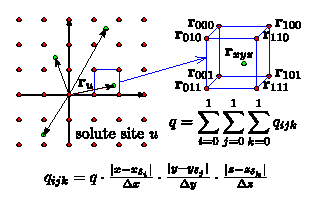
\includegraphics[scale=1.5]{_figure/charge_int_2}
\par\end{centering}
\caption{Solute charge density projected onto grids\label{fig:Charge-density-projected}}
\end{figure}

The electrostatic potential created by the charge distribution $\rho_{q}(\mathbf{r})$,
$V_{q}(\mathbf{r})$, can thus be computed using a periodic Poisson
Solver. The Poisson equation (\ref{eq:poisson})
\begin{equation}
\nabla^{2}V_{q}(\mathbf{r})=-\frac{\rho_{q}(\mathbf{r})}{\varepsilon_{0}}
\end{equation}
gives in Fourier space
\begin{equation}
\hat{V}_{q}(\mathbf{k})=\frac{\hat{\rho}_{q}(\mathbf{k})}{\varepsilon_{0}k^{2}}
\end{equation}
where $\hat{V}_{q}(\mathbf{k})$ and $\hat{\rho}_{q}(\mathbf{k})$
are the Fourier transform of $V_{q}(\mathbf{r})$ and $\rho_{q}(\mathbf{r})$
respectively. These two equations provide a fast way to calculate
$V_{q}(\mathbf{r})$ from $\rho_{q}(\mathbf{r})$.

The Coulomb potential is expressed as a sum of solvent partial charge
contributions at each grid node:
\begin{equation}
V_{\mathrm{coul}}(\mathbf{r},\mathbf{\Omega})=\sum_{v}q_{v}V_{q}(\mathbf{r}_{v})
\end{equation}
where $q_{v}$ is the point charge of solvent, and
\begin{equation}
\mathbf{r}_{v}=\mathbf{r}+\mathbf{R}(\mathbf{\Omega})\mathbf{s}_{v}
\end{equation}
is the Cartesian coordinate of a solvent site $v$; $V_{q}(\mathbf{r}_{u})$
is the electrostatic potential, given by a linear interpolation of
the nearby point of $V_{q}(\mathbf{r})$ obtained in the last step
from the Poisson solver. 

Another method to calculate $V_{\mathrm{coul}}(\mathbf{r},\mathbf{\Omega})$
is direct summation, which gives a non-periodic external potential,
but in the implementation it usually leads to better convergence for
non-spherical molecules. \marginpar{In this thesis we only work on the $\mathcal{F}_{\mathrm{exc}}$
term.}Here we describe its expression, without going into the reason
behind the convergence:
\begin{equation}
V_{\mathrm{coul}}(\mathbf{r},\mathbf{\Omega})=\sum_{u\in\mathrm{solute}}\sum_{v\in\mathrm{solvent}}\left(\dfrac{q_{u}q_{v}}{4\pi\varepsilon_{0}r_{uv}}\right)
\end{equation}
where $r_{uv}$ is calculated as in eq. (\ref{eq:4.ruv}). For
this thesis, the direct summation is only used in the minimization
of non-spherical solutes, specifically in the chapters of implementation and application.

\subsection{The excess term\label{subsec:The-excess-term}}

As shown in $\mathsection$\ref{sec:Classical-density-functional},
we invoke here the \acs{HRF} approximation which amounts to a second-order
Taylor expansion around the homogeneous fluid at density $\rho_{0}$:
\begin{equation}
\mathcal{F}_{\mathrm{exc}}[\rho]=-\frac{k_{B}T}{2}\int\mathrm{d}\mathbf{r}_{1}\mathrm{d}\mathbf{\mathbf{\Omega}}\gamma(\mathbf{r}_{1},\mathbf{\mathbf{\mathbf{\mathbf{\Omega}}}})\rho(\mathbf{r}_{1},\mathbf{\mathbf{\mathbf{\mathbf{\Omega}}}})\label{eq:4.fexc}
\end{equation}
where $\gamma$ is the normalized gradient of the excess functional:
\begin{equation}
\gamma(\mathbf{r}_{1},\mathbf{\Omega}_{1})=-\frac{\delta\beta F_{\mathrm{exc}}}{\delta\rho}=\int\mathrm{d}\mathbf{r}_{2}\mathrm{d}\mathbf{\Omega}_{2}\Delta\rho(\mathbf{r}_{2},\mathbf{\Omega}_{2})c(\mathbf{r}_{12},\mathbf{\Omega}_{1},\mathbf{\Omega}_{2})\label{eq:4.gamma}
\end{equation}
which can be related to the solute-solvent 2-component \acs{IET}
with its definition:
\begin{equation}
\gamma_{\mathrm{MS}}(1,2)=h_{\mathrm{MS}}(1,2)-c_{\mathrm{MS}}(1,2)
\end{equation}

To evaluate the integration $\int\mathrm{d}\mathbf{r}_{2}\mathrm{d}\mathbf{\Omega}_{2}$
for each gradient $\gamma(\mathbf{r}_{1},\mathbf{\Omega}_{1})$ in
eq. (\ref{eq:4.gamma}), a total number of $N^{2}\equiv N_{\mathbf{r}}^{2}N_{\mathbf{\Omega}}^{2}=O(N^{2})$
function evaluations (\acs{FE}) are required, which, with typically
$N_{\mathbf{r}}=64^{3}$ and $N_{\mathbf{\Omega}}=50\sim100$, is
far too costly for current computing technology. For this reason,
Fourier transform is used to treat the spatial convolution.

A convolution
\begin{equation}
h(x_{1})\equiv f(x_{2})\otimes g(x_{2})\equiv\int_{a}^{b}f(x_{2})g(x_{1}-x_{2})dx_{2}\label{eq:convolution-1}
\end{equation}
has the property that
\begin{equation}
\mathfrak{F}[h(x_{1})]=\mathfrak{F}[f(x_{2})]\mathfrak{F}[g(x_{2})]\label{eq:convolution-2}
\end{equation}
$\mathfrak{F}$ being the Fourier transform operation. As $\mathbf{r}_{12}=\mathbf{r}_{1}-\mathbf{r}_{2}$,
eq. (\ref{eq:4.gamma}) is a 3D convolution, which leads to
\begin{equation}
\hat{\gamma}(\mathbf{k},\mathbf{\Omega}_{1})=\int\mathrm{d}\mathbf{\Omega}_{2}\Delta\hat{\rho}(\mathbf{k},\mathbf{\Omega}_{2})\hat{c}(\mathbf{k},\mathbf{\Omega}_{1},\mathbf{\Omega}_{2})\label{eq:4.gamma-k}
\end{equation}
Here we put the hat symbol on the physical quantities to represent
the Fourier transform of their original function.

In eq. (\ref{eq:4.gamma-k}), the integral $\int\mathrm{d}\mathbf{r}_{2}$
of eq. (\ref{eq:4.gamma}) is transformed into a simple product; only
$N_{\mathbf{r}}N_{\mathbf{\Omega}}^{2}$ \acs{FE} are needed to obtain
$\hat{\gamma}(\mathbf{k},\mathbf{\Omega}_{1})$ with given $\Delta\hat{\rho}(\mathbf{k},\mathbf{\Omega}_{2})$.
To this computational cost should be added the transform from $\Delta\rho(\mathbf{r},\mathbf{\Omega})$
to $\Delta\hat{\rho}(\mathbf{k},\mathbf{\Omega})$ and the backward
transform from $\hat{\gamma}(\mathbf{k},\mathbf{\Omega})$ to $\gamma(\mathbf{r},\mathbf{\Omega})$
which are both of order $N_{\mathbf{\Omega}}\cdot O(N_{\mathbf{r}}\log_{2}N_{\mathbf{r}})$
due to the properties of Fast Fourier Transform (\acs{FFT}). The
total number of \acs{FE} is thus reduced from quadratic complexity
$O(N_{\mathbf{r}}^{2}N_{\mathbf{\Omega}}^{2})$ to $N_{\mathbf{r}}N_{\mathbf{\Omega}}^{2}+2N_{\mathbf{\Omega}}\cdot O(N_{\mathbf{r}}\log_{2}N_{\mathbf{r}})=O(N_{\mathbf{r}}\log_{2}N_{\mathbf{r}}N_{\mathbf{\Omega}}^{2})$.
As the total number of spatial grid $N_{\mathbf{r}}$ is of magnitude
$10^{5}\sim10^{6}$, this procedure, which is mathematically equivalent
to the direct evaluation (\ref{eq:4.gamma}), offers a great advantage
in terms of computational efficiency (figure \ref{fig:order-of-growth}
in appendix \ref{chpt:computing-performance}).

The angular-dependent \acs{DCF} of the homogeneous solvent, $\hat{c}(\mathbf{k},\mathbf{\Omega}_{1},\mathbf{\Omega}_{2})$,
is an input data which can be obtained from \acs{MD} or \acs{MC}
simulations. A detailed presentation of the \acs{DCF}s used in this
thesis is available in appendix \ref{chpt:dcf-water}.

\section{Molecular integral equation theory\label{sec:Angular-dependent-iem}}

To adapt the \acs{IET} formalism to non-spherical solvent, Blum \citep{Blum_I,Blum_II,blum_III}
proposed to expand the angle-dependent correlation functions $F(\mathbf{X}_{1},\mathbf{X}_{2})\equiv F(\mathbf{r}_{1},\mathbf{r}_{2},\mathbf{\Omega}_{1},\mathbf{\Omega}_{2})$
onto rotational invariants, such that the \acs{OZ} equation can be
reduced to only a few \acs{FE}. This theory is then adopted by Fries
\& Patey \citep{Fries_Patey_1985}, who proposed a numerical solution
for full \acs{HNC} closure. The test below describes the theory of
Blum, but based on the convention of Fries \& Patey, where Messiah's
definition of generalized spherical harmonics (\acs{GSH}s) is used.
A detailed explication of different conventions of \acs{GSH} is given
in appendix \ref{chpt:symmetry}.

\subsection{Translational and rotational invariance}

If $F$ describes a homogeneous fluid, the translational invariance
($\mathbf{r}_{12}\equiv\mathbf{r}_{1}-\mathbf{r}_{2}$) should be
presented, so then the number of independent variables is reduced from
12 to 9:
\begin{equation}
F(\mathbf{X}_{1},\mathbf{X}_{2})=F(\mathbf{r}_{12},\mathbf{\Omega}_{1},\mathbf{\Omega}_{2})=F(r,\hat{\mathbf{r}}_{12},\mathbf{\Omega}_{1},\mathbf{\Omega}_{2})\label{eq:miet-def-func}
\end{equation}

We can further expand $F$ on Wigner \acs{GSH}s of the three orientations;
then $F$ becomes a sum of an infinite number of projections depending
on $r$ and 8 indices:
\begin{equation}
F(\mathbf{X}_{1},\mathbf{X}_{2})=\sum_{m,n,l=0}^{\infty}\sum_{\left|\mu',\mu\right|\leq m,\left|\nu',\nu\right|\leq n,\left|\lambda'\right|\leq l}F_{\mu'\mu\nu'\nu\lambda'}^{mnl}(r)R_{\mu'\mu}^{m}(\mathbf{\Omega}_{1})R_{\nu'\nu}^{m}(\mathbf{\Omega}_{2})R_{\lambda'0}^{l}(\hat{\mathbf{r}}_{12})
\end{equation}

Assuming that this expansion converges, which is normally the case
for correlation functions, the expansion can be expressed in a limited
number of projections. If we also take into account the rotational
invariance by recombining some terms, only $r$ and 5 independent indices
are necessary to describe all the projections:
\begin{equation}
F_{\mu\nu}^{mnl}(r)=\sum_{\mu'\nu'\lambda'}\left(\begin{array}{ccc}
m & n & l\\
\mu' & \nu' & \lambda'
\end{array}\right)F_{\mu'\mu\nu'\nu\lambda'}^{mnl}(r)
\end{equation}

The projections $F_{\mu\nu}^{mnl}(r)$ with a finite order of expansion
have much fewer terms compared to the angular form in eq. (\ref{eq:miet-def-func})
with the same precision of description.

We can define a basis set of rotational invariant as:
\begin{equation}
\Phi_{\mu\nu}^{mnl}(\mathbf{\Omega}_{1},\mathbf{\Omega}_{2},\mathbf{\hat{r}}_{12})=f^{mnl}\sum_{\mu'\nu'\lambda'}\left(\begin{array}{ccc}
m & n & l\\
\mu' & \nu' & \lambda'
\end{array}\right)R_{\mu'\mu}^{m}(\mathbf{\Omega}_{1})R_{\nu'\nu}^{n}(\mathbf{\Omega}_{2})R_{\lambda'0}^{l}(\mathbf{\hat{r}}_{12})
\end{equation}
where the normalization factor $f^{mnl}$ can be any arbitrary non-zero
constant, depending only on indices $m$, $n$, $l$. In Blum's convention,
it is taken as $\left[\left(2m+1\right)\left(2n+1\right)\right]^{\frac{1}{2}}$.

With these definitions, the relation between the projections and the original
function is:
\begin{equation}
F(\mathbf{X}_{1},\mathbf{X}_{2})=\sum_{mnl\mu\nu}\tilde{F}_{\mu\nu}^{mnl}(r)\Phi_{\mu\nu}^{mnl}(\mathbf{\Omega}_{1},\mathbf{\Omega}_{2},\mathbf{\hat{r}}_{12})
\end{equation}
where $\tilde{F}_{\mu\nu}^{mnl}(r)=F_{\mu\nu}^{mnl}(r)/f^{mnl}$.

\subsection{Blum's reduction of molecular OZ equation}

The molecular Ornstein-Zernike (\acs{MOZ}) equation is defined as:
\begin{equation}
\gamma(\mathbf{X}_{1},\mathbf{X}_{2})=h(\mathbf{X}_{1},\mathbf{X}_{2})-c(\mathbf{X}_{1},\mathbf{X}_{2})=\frac{\rho}{8\pi^{2}}\int\mathrm{d}\mathbf{X}_{3}h(\mathbf{X}_{1},\mathbf{X}_{3})c(\mathbf{X}_{3},\mathbf{X}_{2})\label{eq:4.MOZ}
\end{equation}

The rotational invariant expansion gives:
\begin{equation}
c(\mathbf{X}_{1},\mathbf{X}_{2})=\sum_{mnl\mu\nu}c_{\mu\nu}^{mnl}(r)\Phi_{\mu\nu}^{mnl}(\mathbf{\Omega}_{1},\mathbf{\Omega}_{2},\mathbf{\hat{r}}_{12})
\end{equation}
\begin{equation}
\gamma(\mathbf{X}_{1},\mathbf{X}_{2})=\sum_{mnl\mu\nu}\gamma_{\mu\nu}^{mnl}(r)\Phi_{\mu\nu}^{mnl}(\mathbf{\Omega}_{1},\mathbf{\Omega}_{2},\mathbf{\hat{r}}_{12})
\end{equation}
and also in $k$-space:
\begin{equation}
\hat{c}(\mathbf{k},\mathbf{\Omega}_{1},\mathbf{\Omega}_{2})=\sum_{mnl\mu\nu}\hat{c}_{\mu\nu}^{mnl}(k)\Phi_{\mu\nu}^{mnl}(\mathbf{\Omega}_{1},\mathbf{\Omega}_{2},\mathbf{\hat{k}}_{12})
\end{equation}
\begin{equation}
\hat{\gamma}(\mathbf{k},\mathbf{\Omega}_{1},\mathbf{\Omega}_{2})=\sum_{mnl\mu\nu}\hat{\gamma}_{\mu\nu}^{mnl}(k)\Phi_{\mu\nu}^{mnl}(\mathbf{\Omega}_{1},\mathbf{\Omega}_{2},\mathbf{\hat{k}}_{12})
\end{equation}

The relation between these projections in $r$ and $k$-space is
built by the Hankel transform:
\begin{equation}
\hat{c}_{\mu\nu}^{mnl}(k)=4\pi i^{l}\int\mathrm{d}r\,r^{2}j_{l}(kr)c_{\mu\nu}^{mnl}(r)\label{eq:4.hankel1}
\end{equation}
\begin{equation}
\hat{\gamma}_{\mu\nu}^{mnl}(k)=4\pi i^{l}\int\mathrm{d}r\,r^{2}j_{l}(kr)\gamma_{\mu\nu}^{mnl}(r)\label{eq:4.hankel2}
\end{equation}
where $j_{l}(kr)$ are the spherical Bessel functions of order $l$.
Eq. (\ref{eq:4.hankel1}) and (\ref{eq:4.hankel2}) are built in the
same purpose as eq. (\ref{eq:3.oz-k}) in atomic case, where \acs{FFT}
is used. As an analogue to \acs{FFT}, the fast Hankel transform is
available for such a process. 

Note that if function $f(\mathbf{X}_{1},\mathbf{X}_{2})$ is real
and the molecules processes a symmetry axis $\mathrm{C}_{2v}$, like
water, the projections $f_{\mu\nu}^{mnl}(r)$ are real, therefore
$\hat{f}_{\mu\nu}^{mnl}(k)$ is real if $l$ is even, and pure imaginary
if $l$ is odd. The complete symmetry relations are listed in $\mathsection$\ref{sec:Symmetry-rot_invar}.

The \acs{MOZ} equation based on the rotational invariants $\hat{f}_{\mu\nu}^{mnl}(k)$
can be found in the article of Blum \citep{Blum_I}, but the form
is a bit complicated. To provide a simpler form, Blum defined the $\chi$-transform:
\begin{equation}
\hat{c'}_{\mu\nu,\chi}^{mn}(k)=\sum_{l=\left|m-n\right|}^{m+n}\left(\begin{array}{ccc}
m & n & l\\
\chi & -\chi & 0
\end{array}\right)\hat{c}_{\mu\nu}^{mnl}(k)
\end{equation}
\begin{equation}
\hat{\gamma'}_{\mu\nu,\chi}^{mn}(k)=\sum_{l=\left|m-n\right|}^{m+n}\left(\begin{array}{ccc}
m & n & l\\
\chi & -\chi & 0
\end{array}\right)\hat{\gamma}_{\mu\nu}^{mnl}(k)
\end{equation}
where we use the apostrophe to represent functions in an intermolecular
frame. 

The result \acs{MOZ} equation is:
\begin{equation}
\hat{\gamma'}_{\mu\nu,\chi}^{mn}(k)=\rho\sum_{n_{1}}\sum_{\nu_{1}=-n_{1}}^{n_{1}}(-)^{\chi+\nu_{1}}\left[\hat{\gamma'}_{\mu\nu_{1},\chi}^{mn_{1}}(k)+\hat{c'}_{\mu\nu_{1},\chi}^{mn_{1}}(k)\right]\hat{c'}_{\underline{\nu_{1}}\nu,\chi}^{n_{1}n}(k)
\end{equation}

This simple form of \acs{MOZ} equation reduces the calculation of
$\int\mathrm{d}\mathbf{X}_{3}$ for each $(\mathbf{X}_{1},\mathbf{X}_{2})$
in eq. (\ref{eq:4.MOZ}) to only a sum of terms of $n_{1}$, $\nu_{1}$
for each index of projection.
